% Options for packages loaded elsewhere
\PassOptionsToPackage{unicode}{hyperref}
\PassOptionsToPackage{hyphens}{url}
\PassOptionsToPackage{dvipsnames,svgnames,x11names}{xcolor}
%
\documentclass[
]{article}

\usepackage{amsmath,amssymb}
\usepackage{iftex}
\ifPDFTeX
  \usepackage[T1]{fontenc}
  \usepackage[utf8]{inputenc}
  \usepackage{textcomp} % provide euro and other symbols
\else % if luatex or xetex
  \usepackage{unicode-math}
  \defaultfontfeatures{Scale=MatchLowercase}
  \defaultfontfeatures[\rmfamily]{Ligatures=TeX,Scale=1}
\fi
\usepackage{lmodern}
\ifPDFTeX\else  
    % xetex/luatex font selection
    \setmainfont[]{Latin Modern Roman}
  \setmathfont[]{Latin Modern Math}
\fi
% Use upquote if available, for straight quotes in verbatim environments
\IfFileExists{upquote.sty}{\usepackage{upquote}}{}
\IfFileExists{microtype.sty}{% use microtype if available
  \usepackage[]{microtype}
  \UseMicrotypeSet[protrusion]{basicmath} % disable protrusion for tt fonts
}{}
\makeatletter
\@ifundefined{KOMAClassName}{% if non-KOMA class
  \IfFileExists{parskip.sty}{%
    \usepackage{parskip}
  }{% else
    \setlength{\parindent}{0pt}
    \setlength{\parskip}{6pt plus 2pt minus 1pt}}
}{% if KOMA class
  \KOMAoptions{parskip=half}}
\makeatother
\usepackage{xcolor}
\setlength{\emergencystretch}{3em} % prevent overfull lines
\setcounter{secnumdepth}{5}
% Make \paragraph and \subparagraph free-standing
\makeatletter
\ifx\paragraph\undefined\else
  \let\oldparagraph\paragraph
  \renewcommand{\paragraph}{
    \@ifstar
      \xxxParagraphStar
      \xxxParagraphNoStar
  }
  \newcommand{\xxxParagraphStar}[1]{\oldparagraph*{#1}\mbox{}}
  \newcommand{\xxxParagraphNoStar}[1]{\oldparagraph{#1}\mbox{}}
\fi
\ifx\subparagraph\undefined\else
  \let\oldsubparagraph\subparagraph
  \renewcommand{\subparagraph}{
    \@ifstar
      \xxxSubParagraphStar
      \xxxSubParagraphNoStar
  }
  \newcommand{\xxxSubParagraphStar}[1]{\oldsubparagraph*{#1}\mbox{}}
  \newcommand{\xxxSubParagraphNoStar}[1]{\oldsubparagraph{#1}\mbox{}}
\fi
\makeatother


\providecommand{\tightlist}{%
  \setlength{\itemsep}{0pt}\setlength{\parskip}{0pt}}\usepackage{longtable,booktabs,array}
\usepackage{calc} % for calculating minipage widths
% Correct order of tables after \paragraph or \subparagraph
\usepackage{etoolbox}
\makeatletter
\patchcmd\longtable{\par}{\if@noskipsec\mbox{}\fi\par}{}{}
\makeatother
% Allow footnotes in longtable head/foot
\IfFileExists{footnotehyper.sty}{\usepackage{footnotehyper}}{\usepackage{footnote}}
\makesavenoteenv{longtable}
\usepackage{graphicx}
\makeatletter
\def\maxwidth{\ifdim\Gin@nat@width>\linewidth\linewidth\else\Gin@nat@width\fi}
\def\maxheight{\ifdim\Gin@nat@height>\textheight\textheight\else\Gin@nat@height\fi}
\makeatother
% Scale images if necessary, so that they will not overflow the page
% margins by default, and it is still possible to overwrite the defaults
% using explicit options in \includegraphics[width, height, ...]{}
\setkeys{Gin}{width=\maxwidth,height=\maxheight,keepaspectratio}
% Set default figure placement to htbp
\makeatletter
\def\fps@figure{htbp}
\makeatother
% definitions for citeproc citations
\NewDocumentCommand\citeproctext{}{}
\NewDocumentCommand\citeproc{mm}{%
  \begingroup\def\citeproctext{#2}\cite{#1}\endgroup}
\makeatletter
 % allow citations to break across lines
 \let\@cite@ofmt\@firstofone
 % avoid brackets around text for \cite:
 \def\@biblabel#1{}
 \def\@cite#1#2{{#1\if@tempswa , #2\fi}}
\makeatother
\newlength{\cslhangindent}
\setlength{\cslhangindent}{1.5em}
\newlength{\csllabelwidth}
\setlength{\csllabelwidth}{3em}
\newenvironment{CSLReferences}[2] % #1 hanging-indent, #2 entry-spacing
 {\begin{list}{}{%
  \setlength{\itemindent}{0pt}
  \setlength{\leftmargin}{0pt}
  \setlength{\parsep}{0pt}
  % turn on hanging indent if param 1 is 1
  \ifodd #1
   \setlength{\leftmargin}{\cslhangindent}
   \setlength{\itemindent}{-1\cslhangindent}
  \fi
  % set entry spacing
  \setlength{\itemsep}{#2\baselineskip}}}
 {\end{list}}
\usepackage{calc}
\newcommand{\CSLBlock}[1]{\hfill\break\parbox[t]{\linewidth}{\strut\ignorespaces#1\strut}}
\newcommand{\CSLLeftMargin}[1]{\parbox[t]{\csllabelwidth}{\strut#1\strut}}
\newcommand{\CSLRightInline}[1]{\parbox[t]{\linewidth - \csllabelwidth}{\strut#1\strut}}
\newcommand{\CSLIndent}[1]{\hspace{\cslhangindent}#1}

\usepackage{booktabs}
\usepackage{longtable}
\usepackage{array}
\usepackage{multirow}
\usepackage{wrapfig}
\usepackage{float}
\usepackage{colortbl}
\usepackage{pdflscape}
\usepackage{tabu}
\usepackage{threeparttable}
\usepackage{threeparttablex}
\usepackage[normalem]{ulem}
\usepackage{makecell}
\usepackage{xcolor}
\usepackage{arxiv}
\usepackage{orcidlink}
\usepackage{amsmath}
\usepackage[T1]{fontenc}
\makeatletter
\@ifpackageloaded{caption}{}{\usepackage{caption}}
\AtBeginDocument{%
\ifdefined\contentsname
  \renewcommand*\contentsname{Table of contents}
\else
  \newcommand\contentsname{Table of contents}
\fi
\ifdefined\listfigurename
  \renewcommand*\listfigurename{List of Figures}
\else
  \newcommand\listfigurename{List of Figures}
\fi
\ifdefined\listtablename
  \renewcommand*\listtablename{List of Tables}
\else
  \newcommand\listtablename{List of Tables}
\fi
\ifdefined\figurename
  \renewcommand*\figurename{Figure}
\else
  \newcommand\figurename{Figure}
\fi
\ifdefined\tablename
  \renewcommand*\tablename{Table}
\else
  \newcommand\tablename{Table}
\fi
}
\@ifpackageloaded{float}{}{\usepackage{float}}
\floatstyle{ruled}
\@ifundefined{c@chapter}{\newfloat{codelisting}{h}{lop}}{\newfloat{codelisting}{h}{lop}[chapter]}
\floatname{codelisting}{Listing}
\newcommand*\listoflistings{\listof{codelisting}{List of Listings}}
\makeatother
\makeatletter
\makeatother
\makeatletter
\@ifpackageloaded{caption}{}{\usepackage{caption}}
\@ifpackageloaded{subcaption}{}{\usepackage{subcaption}}
\makeatother
\ifLuaTeX
  \usepackage{selnolig}  % disable illegal ligatures
\fi
\usepackage{bookmark}

\IfFileExists{xurl.sty}{\usepackage{xurl}}{} % add URL line breaks if available
\urlstyle{same} % disable monospaced font for URLs
\hypersetup{
  pdftitle={From Text to Insight - A Novel Approach to Measuring Business Model Innovation},
  pdfauthor={Max Gabler; Wanshu Jiang; Christoph Kiesl; Leonard Pöhls; Alexander Rieber; Ansgar Scherp},
  pdfkeywords={10-K, Business Model Innovation, BERT, Gemini},
  colorlinks=true,
  linkcolor={blue},
  filecolor={Maroon},
  citecolor={Blue},
  urlcolor={Blue},
  pdfcreator={LaTeX via pandoc}}

\newcommand{\runninghead}{A Preprint }
\title{From Text to Insight - A Novel Approach to Measuring Business
Model Innovation}
\def\asep{\\\\\\ } % default: all authors on same column
\author{\textbf{Max
Gabler}\\\href{mailto:max.gabler@uni-ulm.de}{max.gabler@uni-ulm.de}\asep\textbf{Wanshu
Jiang}\\\href{mailto:wanshu.jiang@uni-ulm.de}{wanshu.jiang@uni-ulm.de}\asep\textbf{Christoph
Kiesl}\\\href{mailto:christoph.kiesl@uni-ulm.de}{christoph.kiesl@uni-ulm.de}\asep\textbf{Leonard
Pöhls}\\\href{mailto:leonard.poehls@uni-ulm.de}{leonard.poehls@uni-ulm.de}\asep\textbf{Alexander
Rieber}\\\href{mailto:alexander.rieber@uni-ulm.de}{alexander.rieber@uni-ulm.de}\asep\textbf{Ansgar
Scherp}\\\href{mailto:ansgar.scherp@uni-ulm.de}{ansgar.scherp@uni-ulm.de}}
\date{}
\begin{document}
\maketitle
\begin{abstract}
The ability of companies to continuously innovate and adapt their
business models is a key driver of long-term success in dynamic markets.
In this study, we examine the quantification of business model
innovation (BMI) by means of a text-based analysis of pre-processed 10-K
reports, specifically Item 1 texts that describe companies business
activities. Our approach focuses on two investigations, firstly creating
an industry classification according to Hoberg \& Phillips (2016),
applying a BERT-based (Bidirectional Encoder Representation from
Transformers) similarity index (BERTScore) to text summaries previously
summarized by Google's Gemini. Second, we apply the same approach for
identical firms to capture semantic changes across different years,
while low BERTScores indicate significant changes in the business model
components, which can be interpreted as potential BMI. Our results
provide insights into the extent to which textual similarities in
regulatory reports can be used as a reliable indicator for BMI. This
method could thus represent a novel and scalable approach to analyzing
BMI over time.
\end{abstract}
{\bfseries \emph Keywords}
\def\sep{\textbullet\ }
10-K \sep Business Model Innovation \sep BERT \sep 
Gemini


\renewcommand*\contentsname{Table of contents}
{
\hypersetup{linkcolor=}
\setcounter{tocdepth}{3}
\tableofcontents
}
\newpage{}

\section{Introduction}\label{introduction}

BMI is a key activity to maintain competitiveness and even gain a
competitive advantage (Pucihar et al. 2019; Teece 2018). It is therefore
no surprise that the interest in BMI and methods of measuring it has
grown rapidly over the last twenty years. Researchers have recently
called for a BMI measurement instrument that is more comprehensive and
advanced than already existing ones (Huang and Ichikohji 2023). The
scale developed by Spieth \& Schneider (2016) provides managers and
practitioners with a measurement index for business model
innovativeness. This measurement model only validates applicability of
BMI theory (Huang and Ichikohji 2023) and is insufficient for
longitudinal studies (Clauss 2017). Hence, this measure is not adequate
for a time series analysis of BMI. Furthermore, it refers only to BMI as
new-to-the-firm and is not able to grasp BMI in the sense of
new-to-the-industry and new-to-market. Clauss (2017) developed a similar
measure with comparable limitations.

This gap is addressed by proposing a novel approach to measuring BMI.
US-based companies are obliged by the United States Security and
Exchange Commission (SEC) to submit annual 10-K filings, wherein a
detailed description of the company's business operations is required.
Hoberg \& Phillips (2016) use this filings to create word vectors about
the companies products in order to cluster them into industries and
thereby proposing a new industry classification. This study builds on
their work and methods. We summarize these descriptions with Gemini,
utilize the BERTScore as a similarity measure to calculate the
similarities between companies and cluster them into industries. We
compare our BERTScore clustering with the fixed industry classification
(FIC) by Hoberg \& Phillips (2016). Furthermore, we calculate the
BERTScore between the summaries of different years for a single company.
This approach enables the measurement of changes in the business model
(BM) over time as the distance between the BM summary of one year to
another. There is evidence that an increase in BMI is associated with
improved firm performance (Cucculelli and Bettinelli 2015; Latifi,
Nikou, and Bouwman 2021; White et al. 2022). In order to test the
validity of our measure, we regress financial numbers on our measure,
hoping to find a positive relationship.

\begin{itemize}
\tightlist
\item
  Key findings (and Contribution, already down below)
\end{itemize}

Our contribution is made in two ways. Firstly, we build on the concept
of alternative industry classification put forth by Hoberg \& Phillips
(2016) and propose an industry classification system based on a firm's
BM. Secondly, we propose a novel measure for BMI that is sufficient for
longitudinal studies.

The SEC mandates that the majority of public companies based in the
United States submit specific documents in certain intervals. One such
document is the annual 10-K filing. These filings follow a set order of
topics and contain a range of information, including details about
managerial discussions, risk factors for the company, legal proceedings
and financial data. In the first section under the subtitle
``Business,'' a company presents its general business, encompassing
information about its products and services. In some instances
additional topics may be addressed, such as labor issues or competition
(SEC 2024). In conclusion, this section contains the most useful
information for describing a company's BM (Lee and Hong 2014).
Furthermore, 10-K filings are a reliable source of information, given
that US law prohibits false or misleading statements in the filings. The
SEC monitors the compliance of the companies with the requirements and
comments where disclosure appears to be inconsistent (SEC 2024).

\begin{itemize}
\tightlist
\item
  paragraph 5 (robustness checks)
\end{itemize}

In spite of the growing interest in BMI and the increasing number of
theoretical and empirical studies in this field, the research of BMI is
still in a preliminary state (Huang and Ichikohji 2023). Consequently,
there is considerable variation in the definitions of BMI, with some
definitions being more similar to one another than others (Foss and
Saebi 2017). Spieth \& Schneider (2016) identify three core dimensions a
company's BM is comprised of: its value proposition, its value creation
architecture and its revenue model logic. Based on this, BMI can be
conceptualized as a change that is new-to-the-firm in at least one of
these dimensions. Furthermore, Spieth and Schneider (2016) introduce a
measurement model to evaluate these three dimensions of BMI. They
develop an index by first specifying the contents, followed by a
specification of the indicators and assessing their content validity,
assessing the indicators collinearity and finally assessing the external
validity. A total of twelve indicators for measuring the innovativeness
of the BM were identified through a comprehensive literature review and
through engagement with industry practitioners. The external validity of
the formative indicators was successfully validated through a survey of
200 experts in strategy and innovation management (Spieth and Schneider
2016). Clauss (2017) employs a very similar approach. After specifying
the domain and dimensionality of BMI trough literature research, the
author divides his scale into three hierarchical levels consisting of 41
reflective items, 10 subconstructs and three main dimensions, which are
similar to the ones mentioned earlier. The scale was validated through
two samples from the manufacturing industry and further demonstrated
nomological validity (Clauss 2017). However, both measures are subject
to three significant limitations. Firstly, both measures lack a temporal
component. Consequently, they are inadequate for use in longitudinal
studies or ex-post evaluations of BMI. Secondly, BMI is only measured at
the new-to-the-firm level rather than at the new-to-the-industry or
new-to-the-market level. Thirdly, both measures rely on interviews and
questionnaires, which makes conducting large-scale studies
time-consuming and reliant on the willingness of the companies to
cooperate (Clauss 2017; Spieth and Schneider 2016).

The process of text mining 10-K filings is not a novel concept. Hoberg
\& Phillips (2016) present a novel approach to defining industry
boundaries. This is achieved through the parsing of the product
descriptions provided by firm 10-K filings and creating word vectors.
Specifically, the authors identify and exclude proper nouns, which
include common words and geographic locations. They then create word
vectors for each firm and year, which enables the measurement of product
similarity over time. They propose two novel industry classification
methods: the FIC and the text-based network industry classification
(TNIC). Firstly, they cluster companies based on the similarity of the
word vectors into fixed industries. Secondly, they define a minimum
similarity threshold, above which firms are considered in the same
industry. This relaxes their prior properties of binary membership
transitivity and fixed industry location. This way the authors
demonstrate shortcomings in the traditional industry classification
systems such as the Standard Industry Classification (SIC) and the North
American Industry Classification System (NAICS), which are not able to
account for temporal changes. The new method is capable of capturing
changes in industry boundaries and competitor sets over time, thereby
providing a dynamic industry classification system. In their study, Lee
\& Hong (2014) examine the evolution of a firm's BM over time. The
authors represent each document as a vector of keywords, which is
similar to the approach utilized by Hoberg \& Phillips (2016). After
identifying the Item 1 part of the 10-K filings as the most crucial part
for describing a firm's BM, Lee \& Hong (2014) filter these for relevant
sentences. Subsequently, the authors construct keyword vectors, which
represent the concept of the BM. Therefore, the evolution of the BM is
depicted as the change in the distribution of keywords over time.
Nevertheless, this approach is not without shortcomings. The authors
advocate for a more robust methodology, such as incorporating multi-word
phrases in the keyword vectors, to enhance the reliability of the
approach (Lee and Hong 2014).

The rest of the paper proceeds as follows. Section 2 describes the
preprocessing with Gemini, our data and our methodology. Section 3
compares the industry classification based on product descriptions by
Hoberg \& Phillips (2016) with our classification based on the BM.
Section 4 lays out the BERT-model and our estimations. Section 5
discusses our results, and Section 6 concludes our study.

\newpage{}

\section{Data and Methodology}\label{data-and-methodology}

\subsection{Preprocessing with Gemini}\label{preprocessing-with-gemini}

10-K filings are typically very large text documents, and Item 1 of
these filings is no exception. Table 1 shows the descriptive measures of
the length of the original Item 1 section in our final sample. The
length of a document was measured by the word count without punctuation.
The document length ranges from a couple hundred words to tens of
thousands. In order to utilise the entirety of the information regarding
the BM in the Item 1 section and pass the text to our BERT model, we
decided to let Google's GenAI chatbot Gemini summarize them to a maximum
length of 512 tokens. The summaries were created between 26 June 2024
and 6 August 2024. The model employed was Gemini Flash 1.5. The prompt
was inserted at the beginning of each text file and it was passed via an
API to Gemini \footnote{We forked and used following Github Repository:
  https://github.com/skranz/gemini\_ex.}. We used following prompt:
``Summarize the business model from the following text. Answer with a
continuous text and with five hundred twelve tokens at max. Set your
focus on sources of revenue, the intended customer base, products,
distribution channels and details of financing. Use only information
from the following the text''.\footnote{The spelling error in the last
  sentence of the prompt was found after processing Item 1. After
  evaluating the Summaries, this error did not cause any issues.}
``intended customer base'' and ``product'' refer to the value offering,
``distribution channels'' refers to the value architecture, and
``sources of revenue'' and ``details of financing'' refer to the revenue
model. Consequently, this prompt covers all aspects of the definition of
BMI proposed by Spieth \& Schneider (2016). The term `tokens' was used
deliberately in preference to `words', given that the number of tokens
and the number of words in a text may vary depending on the tokeniser.
This way, we wanted to ensure that the whole summary is used by the BERT
model. To assess the quality and accuracy of the summaries produced by
Gemini, a random sample of 100 filings was selected for comparison with
the original text. More precise,the original file was initially read
with a focus on the points mentioned in the prompt. Subsequently, the
summary was evaluated to ascertain whether it contained these same
points. A list of the sample with the summaries is provided in the
Appendix.

\begin{itemize}
\tightlist
\item
  result of this check
\end{itemize}

\begin{figure}

\begin{minipage}{\linewidth}

\begin{longtable}[]{@{}
  >{\raggedleft\arraybackslash}p{(\columnwidth - 14\tabcolsep) * \real{0.0588}}
  >{\raggedleft\arraybackslash}p{(\columnwidth - 14\tabcolsep) * \real{0.0706}}
  >{\raggedleft\arraybackslash}p{(\columnwidth - 14\tabcolsep) * \real{0.2235}}
  >{\raggedleft\arraybackslash}p{(\columnwidth - 14\tabcolsep) * \real{0.0941}}
  >{\raggedleft\arraybackslash}p{(\columnwidth - 14\tabcolsep) * \real{0.1882}}
  >{\raggedleft\arraybackslash}p{(\columnwidth - 14\tabcolsep) * \real{0.0824}}
  >{\raggedleft\arraybackslash}p{(\columnwidth - 14\tabcolsep) * \real{0.1882}}
  >{\raggedleft\arraybackslash}p{(\columnwidth - 14\tabcolsep) * \real{0.0941}}@{}}
\caption{Descriptive Statistics Original Filings}\tabularnewline
\toprule\noalign{}
\begin{minipage}[b]{\linewidth}\raggedleft
Year
\end{minipage} & \begin{minipage}[b]{\linewidth}\raggedleft
Mean
\end{minipage} & \begin{minipage}[b]{\linewidth}\raggedleft
Standard Deviation
\end{minipage} & \begin{minipage}[b]{\linewidth}\raggedleft
Minimum
\end{minipage} & \begin{minipage}[b]{\linewidth}\raggedleft
25th Percentile
\end{minipage} & \begin{minipage}[b]{\linewidth}\raggedleft
Median
\end{minipage} & \begin{minipage}[b]{\linewidth}\raggedleft
75th Percentile
\end{minipage} & \begin{minipage}[b]{\linewidth}\raggedleft
Maximum
\end{minipage} \\
\midrule\noalign{}
\endfirsthead
\toprule\noalign{}
\begin{minipage}[b]{\linewidth}\raggedleft
Year
\end{minipage} & \begin{minipage}[b]{\linewidth}\raggedleft
Mean
\end{minipage} & \begin{minipage}[b]{\linewidth}\raggedleft
Standard Deviation
\end{minipage} & \begin{minipage}[b]{\linewidth}\raggedleft
Minimum
\end{minipage} & \begin{minipage}[b]{\linewidth}\raggedleft
25th Percentile
\end{minipage} & \begin{minipage}[b]{\linewidth}\raggedleft
Median
\end{minipage} & \begin{minipage}[b]{\linewidth}\raggedleft
75th Percentile
\end{minipage} & \begin{minipage}[b]{\linewidth}\raggedleft
Maximum
\end{minipage} \\
\midrule\noalign{}
\endhead
\bottomrule\noalign{}
\endlastfoot
2016 & 7842 & 6104 & 155 & 3705 & 6026 & 10271 & 51227 \\
2017 & 7542 & 6320 & 155 & 3522 & 5767 & 9700 & 70611 \\
2018 & 7604 & 6272 & 180 & 3528 & 5771 & 9669 & 71700 \\
2019 & 8009 & 6631 & 189 & 3669 & 5971 & 10410 & 78270 \\
2020 & 8660 & 7195 & 171 & 3943 & 6449 & 10971 & 57980 \\
2021 & 10324 & 8406 & 235 & 4670 & 7568 & 13563 & 78799 \\
2022 & 9471 & 7997 & 171 & 4309 & 7042 & 11897 & 73937 \\
2023 & 6646 & 4771 & 190 & 3660 & 5814 & 8401 & 43523 \\
\end{longtable}

\end{minipage}%

\end{figure}%

\subsection{The Dataset}\label{the-dataset}

We collect 10-K filings from the digital SEC Database, using the
category ``10-K'' as extraction condition. Since the focus of our study
lies on company's BM, we merely use the Item 1 part, since this is the
most crucial part of the 10-K filings for describing the companies BM
(Lee and Hong 2014). Our observations are limited to an intersection of
such companies, which on the one hand has been made available to the SEC
since 2001 in a publicly accessible list of 10,284 companies (Appendix),
of which 7,590 are currently listed on NASDAQ, NYSE or over-the-counter.
We extracted 10-K filings that were submitted between 2017 and 2023
based on underlying Central Index Keys (CIK). We exclude companies from
the financial sector, namely companies with a SIC Code starting with
six. Corresponding to Table 2, multiple steps of pre-processing were
required to obtain a final amount 21,683 observations of seven years.
Financial key figures, including net income, total assets and others
were originally extracted from the SEC, but also challenged with
financial values from DataStream. A total of 4,225 companies are
included in the sample, although the availability of filings could not
always be guaranteed for all years. This is due on the one hand to the
quality of the API to the SEC and on the other hand to companies that
did not file 10-K reports or were listed on the stock exchange for the
entire period under review. Finally, we have access to the financial key
figures of the companies for the respective year, the Item I text
pre-processed with the help of Gemini, company-specific identification
features and the conventional SIC industry classification.

\begin{figure}

\begin{minipage}{\linewidth}

\begin{longtable}[t]{>{\raggedright\arraybackslash}p{8cm}rl}
\caption{10-K Sample Creation}\tabularnewline

\toprule
Source/Filter & Sample Size & Observations Removed\\
\midrule
1. Extracted 10-K filings from the SEC & 35731 & \\
2. Excluding filings from financial companies (SIC-code starting with '6') & 27569 & 8162\\
3. Verify for Item 1 text availability (removed oberservations that are attributable to API quality) & 23982 & 3587\\
4. Extracting dates for which the filings are reporting for and removing of duplicated filings & 23971 & 11\\
5. Delete observations with incorrect date assignment & 22161 & 1810\\
\addlinespace
6. Merged Gemini processed Item 1 text to the underlying data set. We did not consider texts that were not processable & 21697 & 464\\
7. Extract financials statements from SEC and merge them. Also remove observations for years prior to 2016 & 21686 & 11\\
\bottomrule
\multicolumn{3}{l}{\rule{0pt}{1em}\textit{Note: }}\\
\multicolumn{3}{l}{\rule{0pt}{1em}Filings submitted between 2017 and 2023 are considered}\\
\end{longtable}

\end{minipage}%

\end{figure}%

TODO

\begin{itemize}
\tightlist
\item
  Descriptive Table3 for length of summary (in words and tokens (use
  tokenizer our Model uses))
\item
  Description of Table2, Table3, and the final dataset
\item
  something (Table, Figure) for looking at distribution of BERTScore
\end{itemize}

\subsection{Methodology}\label{methodology}

After processing the data, we calculate the BERTScore between the
summaries of different companies and between the summaries for the same
company of different years. The similarity between different companies
in the same year is utilized in Section 3 to compare the FIC by Hoberg
\& Phillips (2016) with the industry classification by the BERTScore.

hoberg use word vectors and product description, we use BERT and
everything regarding the BMI, different object ob research. By
definition of spieth is the product a part of the value offering,
thereby a part of the BMI. Because product is thereby entangled, we
expect a similar distribution as Hoberg for the FIC. very granular, lot
of small industries. This motivates H1 and H2:

\textbf{H1}: We expect a similar distribution of firms.

\textbf{H2}: We expect a high overlap with Hobergs classification.

focus will not be an the replication because our approach differs very
strong from original paper. We not only calc similarity between
different firms, but also for the same firm over time. this allows
measuring the change in BM. Under the assumption that companies ``don't
run in circles'', this measures BMI on the new to the firm level. in
literature, positive relationship between BMI and firm performance is
explored. to test our measure, we regress firm performance on BMI (and
other controlls found in the literature). When 1-BERTScore really
measures BMI, we expect H3 to be true:

\textbf{H3}: Our measure for BMI shows a positive relationship with firm
performance

\section{Replication}\label{replication}

Our study builds on the idea of Hoberg \& Phillips (2016) to utilize
text data from 10-K filings to classify companies based on their
similarity to each other into dynamic industries. Our approach differs
in two ways: Firstly, in contrast to the TNIC and FIC, which employ
word-to-vec, our approach utilises BERT to represent text. Accordingly,
the BERTScore is employed instead of the cosine similarity as our
similarity measure. Secondly, our analysis is focused on the description
of the BM rather than on the product descriptions. In order to set a
benchmark for our BERTScore industry classification, we have replicated
the FIC approach as described by Hoberg \& Phillips (2016).
Subsequently, a comparison is made between the industry classification
produced in this study and the aforementioned benchmark.

The data employed for the industry classification with the BERTScore is
the same as described in Section 2. In order to establish a benchmark,
we have utilised the similarity scores provided by Hoberg-Phillips Data
Library.\footnote{For the database see:
  https://hobergphillips.tuck.dartmouth.edu.} The data consists of the
gvkeys of two companies, the year and the cosine similarity between
these two companies. In order to ensure comparability, only companies
present in both the present study's dataset and that provided by the
authors are included in the analysis. Because we use CIKs and accession
numbers to identify firms and filings, and the fact that the data
library employs Compustat's gvkeys, the matching of CIKs with gvkeys
inevitably results in the loss of some observations. Ultimately, the
clustering algorithm was applied to 1,958 firms for the year 2017.
Hoberg \& Phillips (2016) perform two steps to create the FIC. Firstly,
a hierarchical agglomerative clustering algorithm is employed to cluster
companies based on their similarity and maximize ex-post within cluster
similarity. This enables a classification with any number of clusters.
They perform this step in increments of 50, but focus on 300 industries
since this is very analogous to the number of industries of the SIC and
the NAICS. Therefore, a comparison is made between our industry
classification and the FIC based on 300 industries. In the second step,
the authors compute aggregated word vectors for each industry. These
vectors now represent the industries. Subsequently, the similarity
between industries and firms is calculated for each of the following
years. From the second year onwards, firms are classified according to
the industry with which they are most similar. The FIC satisfies the
binary membership transitivity property and the fixed location property.
The binary membership transitivity property states that if two firms are
in the same industry and a third firm is in the same industry as one of
the other two, then it is also in the same industry as the other. The
fixed location property dictates that clusters are not recalculated on
an annual basis, but rather remain fixed until the codes are
updated.(Hoberg and Phillips 2016).

Figure 1 compares the distribution of industry size for the BERTScore
classification and the FIC The BERTScore classification shows a similar
picture as the FIC Both are left skewed, with most industries being
smaller than ten firms. The distribution of the FIC is steeper than the
on of the BERTScore classification. It is noteworthy, that the largest
industry in the BERTScore classification only consists of 27 companies,
while the FIC contains industries larger than this, with some over 50
companies. This indicates that the BERTScore classification clusters
small to medium sized industries ranging between two to fourteen firms
per industry with less large industries. The FIC also consists mostly of
small to medium, but also a few large industries. Despite these minor
differences, this supports H1.

Regarding H2: Medium Homogeneity with 0.63 and Medium Completeness with
0.6026; Low Adjusted Rand Index (ARI) with 0.0002 and low
Fowlkes-Mallows Index (FMI) -\textgreater{} indicates clusters are not
better than random; No support for H2; Reason could be different object
of investigation (BM vs product description)

The industries in the FIC are fixed, but by dropping the fixed location
property, the industry classification are time-varying. Furthermore, if
the binary membership transitivity property is relaxed, the result is
the TNIC by Hoberg \& Phillips (2016). The removal of the fixed location
property encourages the notion of not fixing a specific year and
calculating the similarities between different companies, but rather
fixing a company and calculating the similarity between this firm and
others over time.Such considerations result in a shift in focus away
from industry classification towards an analysis of a company's
evolution. As previously stated, 10-K filings are rich on information
and contain a wealth of data beyond mere product descriptions. The
additional information can be leveraged to investigate a company's BM.
The combination of both rationales -- fixing a company over time and
analysing the BM -- constitutes the primary concept of this study.

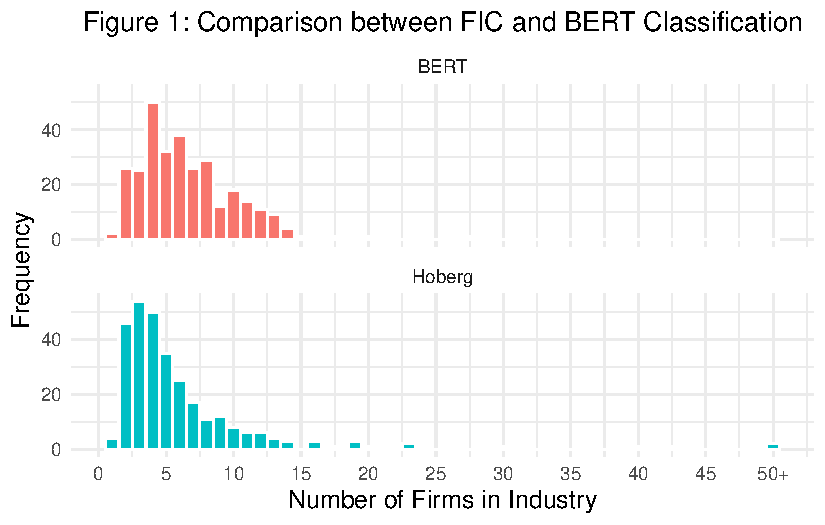
\includegraphics{ProjectEcoDataScience_files/figure-pdf/unnamed-chunk-4-1.pdf}

\section{Empirical Framework}\label{empirical-framework}

The definition of BM includes according to Spieth \& Schneider (2016)
the three components value proposition, value creation and its revenue
model logic. We used the pre-processing of Item I texts with Gemini to
control these texts using a specific prompt in that the focus of the
texts is on the definition of these three components. Hence, our
BERT-based similarity scores between processed texts represent an index
for BMI that can be used for empirical studies. A preliminary validity
check of these similarity scores should be performed.

\subsection{BERT and BERTScore}\label{bert-and-bertscore}

BERT is a pre-trained and transformer-based model for natural language
processing (NPL) based on artificial neural networks. It works according
to the so-called transformer architecture, which was first mentioned by
Vaswani et. al (2017) {[}\ldots.{]}. According to these authors, this
architecture consists of two main components, the encoder and the
decoder. The encoder consists of several identical layers, which
initially use the so-called self-attention mechanism to generate
context-dependent representations of each word in the sentence. This
mechanism can be parallelized and therefore enables different aspects of
the context to be captured in the same way. The decoder, on the other
hand, works in a similar way and is responsible for processing the
information from the encoder and forming it into an output sequence.
However, this is not relevant for BERT, as no sequence-to-sequence
transformation is carried out in BERT. In contrast to Hoberg \& Philips
(2016) (2016) word-to-vec approach, BERT works bidirectional and takes
into account the context from both sides of each word simultaneously.
Therefore, BERT is able to capture deeper semantics in texts such as
10-K reports. The BERTScore now computes the cosine similarity between
word or text meanings, that have been determined by representations (or
embeddings) learned from BERT. The scale is from -1 to 1, where 1
describes a perfect similarity.

\subsection{Estimation Strategy}\label{estimation-strategy}

\section{Results and Discussion}\label{results-and-discussion}

\section{Conclusion}\label{conclusion}

\section{Acknowledgement}\label{acknowledgement}

\begin{itemize}
\tightlist
\item
  Jonathan for IT Support
\item
  Prof.~Kranz for Repo
\end{itemize}

\newpage{}

\section{References}\label{references}

\phantomsection\label{refs}
\begin{CSLReferences}{1}{0}
\bibitem[\citeproctext]{ref-clauss_measuring_2017}
Clauss, Thomas. 2017. {``Measuring Business Model Innovation:
Conceptualization, Scale Development, and Proof of Performance.''}
\emph{R\&D Management} 47 (3): 385--403.
\url{https://doi.org/10.1111/radm.12186}.

\bibitem[\citeproctext]{ref-cucculelli_business_2015}
Cucculelli, Marco, and Cristina Bettinelli. 2015. {``Business Models,
Intangibles and Firm Performance: Evidence on Corporate Entrepreneurship
from {Italian} Manufacturing {SMEs}.''} \emph{Small Business Economics}
45 (2): 329--50. \url{https://doi.org/10.1007/s11187-015-9631-7}.

\bibitem[\citeproctext]{ref-foss_fifteen_2017}
Foss, Nicolai J., and Tina Saebi. 2017. {``Fifteen {Years} of {Research}
on {Business} {Model} {Innovation}: {How} {Far} {Have} {We} {Come}, and
{Where} {Should} {We} {Go}?''} \emph{Journal of Management} 43 (1):
200--227. \url{https://doi.org/10.1177/0149206316675927}.

\bibitem[\citeproctext]{ref-hoberg_text-based_2016}
Hoberg, Gerard, and Gordon Phillips. 2016. {``Text-{Based} {Network}
{Industries} and {Endogenous} {Product} {Differentiation}.''}
\emph{Journal of Political Economy} 124 (5): 1423--65.
\url{https://doi.org/10.1086/688176}.

\bibitem[\citeproctext]{ref-huang_review_2023}
Huang, WenJun, and Takeyasu Ichikohji. 2023. {``A Review and Analysis of
the Business Model Innovation Literature.''} \emph{Heliyon} 9 (7):
e17895. \url{https://doi.org/10.1016/j.heliyon.2023.e17895}.

\bibitem[\citeproctext]{ref-latifi_business_2021}
Latifi, Mohammad-Ali, Shahrokh Nikou, and Harry Bouwman. 2021.
{``Business Model Innovation and Firm Performance: {Exploring} Causal
Mechanisms in {SMEs}.''} \emph{Technovation} 107 (September): 102274.
\url{https://doi.org/10.1016/j.technovation.2021.102274}.

\bibitem[\citeproctext]{ref-lee_business_2014}
Lee, Jihwan, and Yoo S. Hong. 2014. {``Business {Model} {Mining}:
{Analyzing} a {Firm}'s {Business} {Model} with {Text} {Mining} of
{Annual} {Report}.''} \emph{Industrial Engineering and Management
Systems} 13 (4): 432--41.
\url{https://doi.org/10.7232/iems.2014.13.4.432}.

\bibitem[\citeproctext]{ref-pucihar_drivers_2019}
Pucihar, Andreja, Gregor Lenart, Mirjana Kljajić Borštnar, Doroteja
Vidmar, and Marjeta Marolt. 2019. {``Drivers and {Outcomes} of
{Business} {Model} {Innovation}---{Micro}, {Small} and {Medium}-{Sized}
{Enterprises} {Perspective}.''} \emph{Sustainability} 11 (2): 344.
\url{https://doi.org/10.3390/su11020344}.

\bibitem[\citeproctext]{ref-sec_investor_2024}
SEC. 2024. {``Investor {Bulletin}: {How} to {Read} a 10-{K}.''}
\url{https://www.sec.gov/files/reada10k.pdf}.

\bibitem[\citeproctext]{ref-spieth_business_2016}
Spieth, Patrick, and Sabrina Schneider. 2016. {``Business Model
Innovativeness: Designing a Formative Measure for Business Model
Innovation.''} \emph{Journal of Business Economics} 86 (6): 671--96.
\url{https://doi.org/10.1007/s11573-015-0794-0}.

\bibitem[\citeproctext]{ref-teece_business_2018}
Teece, David J. 2018. {``Business Models and Dynamic Capabilities.''}
\emph{Long Range Planning} 51 (1): 40--49.
\url{https://doi.org/10.1016/j.lrp.2017.06.007}.

\bibitem[\citeproctext]{ref-white_exploring_2022}
White, Joshua V., Erik Markin, David Marshall, and Vishal K. Gupta.
2022. {``Exploring the Boundaries of Business Model Innovation and Firm
Performance: {A} Meta-Analysis.''} \emph{Long Range Planning} 55 (5):
102242. \url{https://doi.org/10.1016/j.lrp.2022.102242}.

\end{CSLReferences}

\newpage{}

\section{Appendix}\label{appendix}



\end{document}
